\chapter{Implementierungsplan}
\label{ch:implplan}
Um einen Implementierungsplan aufzustellen wurde das Projekt zuerst anhand der einzelnen Plugins/Pakete und dann noch feiner in einzelne möglichst voneinander unabhängige Aufgaben unterteilt. Der benötigte Arbeitsaufwand zum Bearbeiten der Aufgaben wurden von allen Projektmitgliedern abgeschätzt und deren Mittelwert als geplante Bearbeitungsdauer zur Fertigstellung der Aufgabe angenommen. Anhand von bestehenden Abhängigkeiten der Aufgaben untereinander und der vorausgesetzten wöchentlichen Arbeitsleistung wurden die Aufgaben auf die einzelnen Wochen und Personen verteilt. \\
\begin{figure}[!htbp]
	\centering
	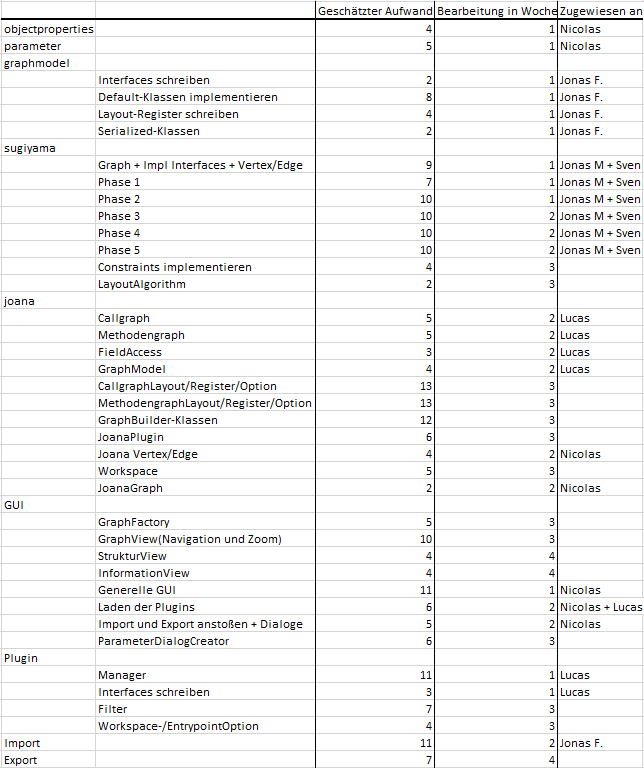
\includegraphics[width=300pt]{week_zero_table.PNG}
	\caption{Erster Implementierungsplan}
	\label{fig:week_zero_table}
\end{figure}
\newpage
\section{Woche 1}
In der ersten Woche wurde der zuerst erstellte Implementierungsplan komplett überarbeitet. Dies war nötig da im ersten Plan viele Abhängigkeiten zwischen den Aufgaben nicht berücksichtigt wurden. Zum Beispiel hing das restliche Projekt komplett von der Fertigstellung des Sugiyama ab und hätte ohne diese nicht getestet werden können. Um dieses Problem zu lösen wurden vorläufige Mockups für die einzelnen Phasen eingeplant. Die anderen Aufgaben wurden zusätzlich in der Abarbeitungsreihenfolge umsortiert, verfeinert und für die ersten zwei Wochen einzelnen Personen zugewiesen. Außerdem wurde eine Tabelle erstellt, die den bereits existierenden Plan, durch eine Fortschrittsspalte, in der die Entwickler ihren Prozentualen Fortschritt der ihnen zugeteilten Aufgaben eintragen, und eine visuelle Repräsentation des Soll- und Ist-Zustands des gesamten Projekt erweitert.\\
\\
Zusätzlich zur Änderung des Plans wurde eine grobe Projektstruktur in Gradle aufgebaut und die bereits im Entwurf gemachten Interfaces in das Projekt überführt. Um die Gradle Projektkonfiguration zu testen wurde eine grobe GUI implementiert und die Entwicklung der allgemeinen genutzten Klassen aus dem Paket "graphmodel"  begonnen.

\begin{figure}[!htbp]
	\centering
	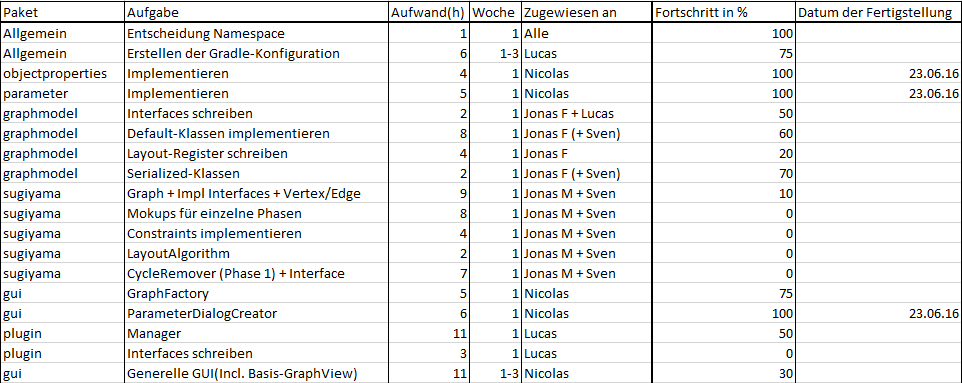
\includegraphics[width=380pt]{week_one_table.PNG}
	\caption{Überarbeiteter Plan für Woche 1 mit Fortschritt}
	\label{fig:week_one_table}
\end{figure}

\subsection{Verzögerungen}
Wie man in \ref{fig:week_one_diagram} sehen kann hing das Projekt nach der ersten Woche bereits ca. 35 Stunden hinter dem geplanten Zustand hinterher.
Dies lag neben der Tatsache das die erste Hälfte der Woche, auf Grund von Erschöpfung aus der Entwurfsphase, weniger gearbeitet wurde, auch daran, dass das Team das für die Implementierung des Sugiyama-Layoutalgorithmus eingeteilt wurde relativ schnell auf konzeptionelle Probleme mit dem im Entwurf definierten Aufbau des SugiyamaGraphen und dessen Kanten/Knoten stieß(siehe \ref{sec:change_sugiyama}).

\begin{figure}[!htbp]
	\centering
	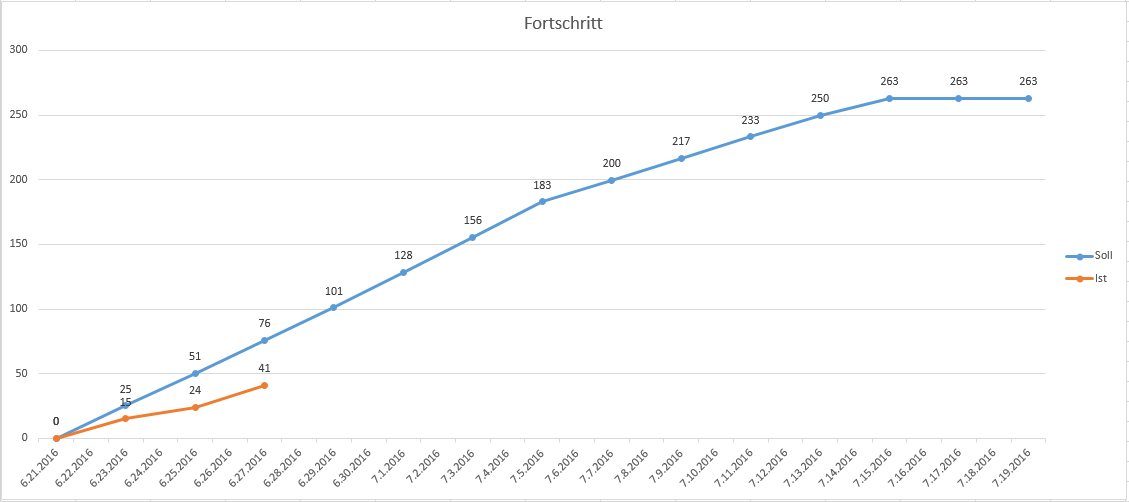
\includegraphics[width=380pt]{resourcen/week_one_diagram.PNG}
	\caption{Fortschrittsdiagramm nach Woche 1}
	\label{fig:week_one_diagram}
\end{figure}
\newpage

\section{Woche 2}
In Woche 2 wurde vorrangig daran gearbeitet einen Graphen einzulesen, mit den im Sugiyama implementierten Klassen oder Mockups zu layouten und in der Anzeige darzustellen. Dazu wurde besonders auf die zeitnahe Fertigstellung des Imports und das funktionsfähig machen des JOANA-Graph-Plugins mit allen dazugehörigen Klassen geachtet. Zudem wurde auch in den Phasen des Sugiyama-Algorithmus große Fortschritte gemacht und manche sogar abgeschlossen. Dadurch entstand der, wie in \ref{fig:week_two_diagram} zu sehen ist, sprunghafte Anstieg des Fortschritts der Fast bis an den Soll-Wert heran reicht. 
\begin{figure}[!htbp]
	\centering
	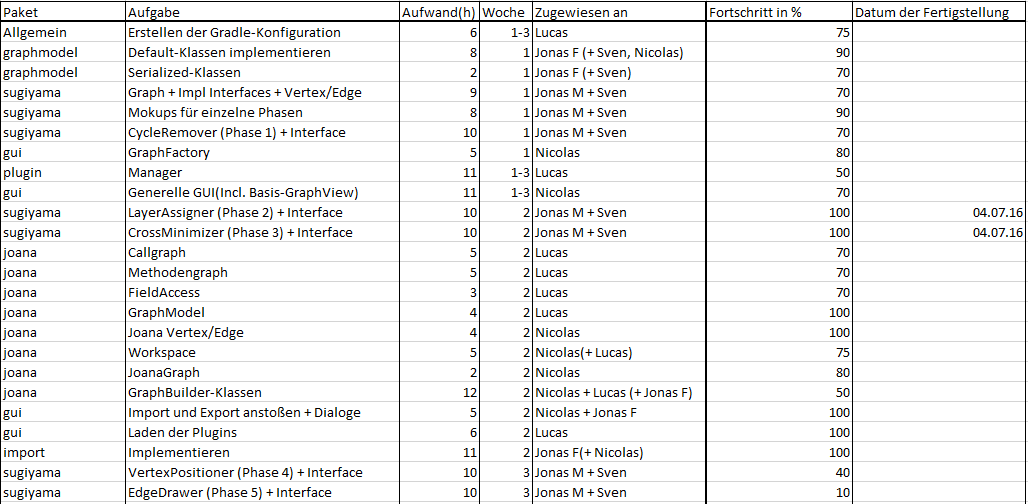
\includegraphics[width=380pt]{week_two_table.PNG}
	\caption{Implementierungsplan für Woche 1 und 2 mit Fortschritt}
	\label{fig:week_two_table}
\end{figure}
\subsection{Verzögerungen}
\label{sec:delay_week2}
Aufgrund der im Entwurf definierten Generics im GraphModel entstanden häufig sehr unschöne Stellen im Code und Inkompatibilitäten. Diese zu reparieren oder funktionsfähig zu machen war häufig Grund für mehr oder weniger unschöne Workarounds die Teilweise viel Arbeit in Anspruch nahmen. Deshalb wurde im Laufe der folgenden Woche ein großes Refactoring vorgenommen welches die Generic-Struktur im GraphModel stark vereinfachte.

\begin{figure}[!htbp]
	\centering
	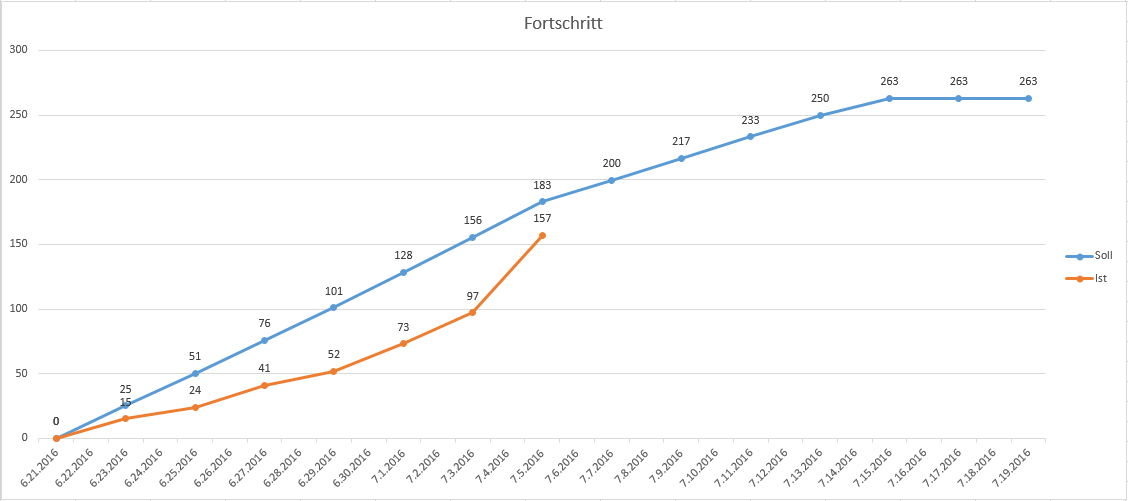
\includegraphics[width=380pt]{resourcen/week_two_diagram.PNG}
	\caption{Fortschrittsdiagramm nach Woche 2}
	\label{fig:week_two_diagram}
\end{figure}

\section{Woche 3}
In Woche 3 wurde das in \ref{sec:delay_week2} beschriebene Refactoring vorgenommen. Dazu wurden die letzten zwei Phasen des Sugiyama benutzbar gemacht und die Oberfläche weiter verfeinert.
\begin{figure}[!htbp]
	\centering
	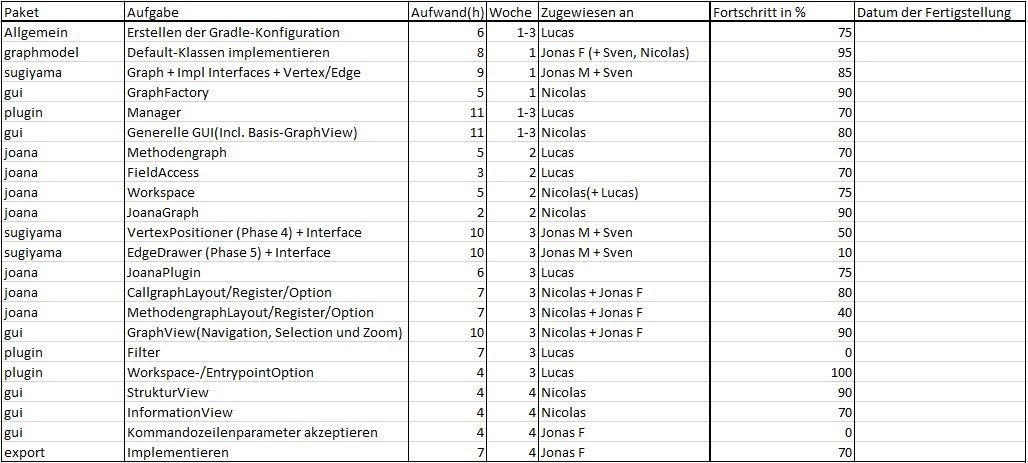
\includegraphics[width=380pt]{week_three_table.PNG}
	\caption{}
	\label{fig:week_three_table}
\end{figure}
\subsection{Verzögerungen}
Nach dem Sprint zum Ende der zweiten Woche wurde wie in \ref{fig:week_three_diagram} zu sehen ist zunächst weniger gearbeitet, ab Mitte der Woche wurde aber wieder der normale Arbeitsrythmus aufgenommen und es kam zu keinen Verzögerungen mehr.
\begin{figure}[!htbp]
	\centering
	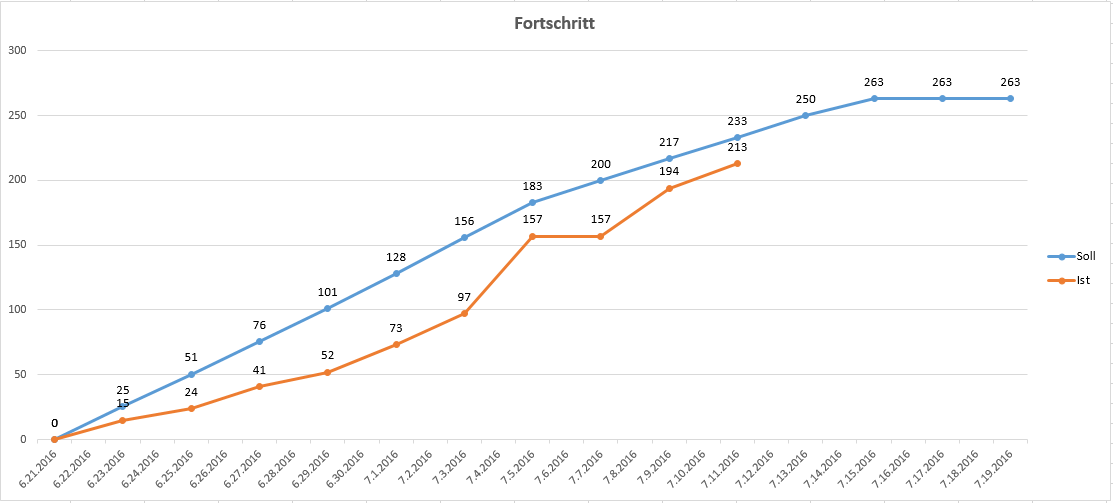
\includegraphics[width=380pt]{resourcen/week_three_diagram.PNG}
	\caption{Fortschrittsdiagramm nach Woche 3}
	\label{fig:week_three_diagram}
\end{figure}
\section{Woche 4}
Am Ende der 4. Woche muss man Rückblickend sagen das der Implementierungsplan zwar von seiner Struktur und den generellen zeitlichen Abschätzung her gut war, der Arbeitsaufwand aber bei vielen Aufgabenbereichen stark unterschätzt wurde. Das lag häufig daran das im Entwurf gemachte Designentscheidungen vermutlich nicht tief genug durchdacht waren und im Laufe der Entwicklung angepasst oder komplett neu erdacht werden mussten. Diese Anpassungen haben an verschiedenen Stellen sehr viel Zeit in Anspruch genommen die nicht im Implementierungsplan vermerkt wurde. Die Verzögerungen spiegeln sich besonders in der flachen Fortschrittskurve in den ersten zwei Wochen dar und haben die gesamte Entwicklung zurückgeworfen hat.
